% SOURCE: ../../edit-harness/results/frame_a/cells/cell_*_real_MIX_A_*.json
% !TEX encoding = UTF-8 Unicode
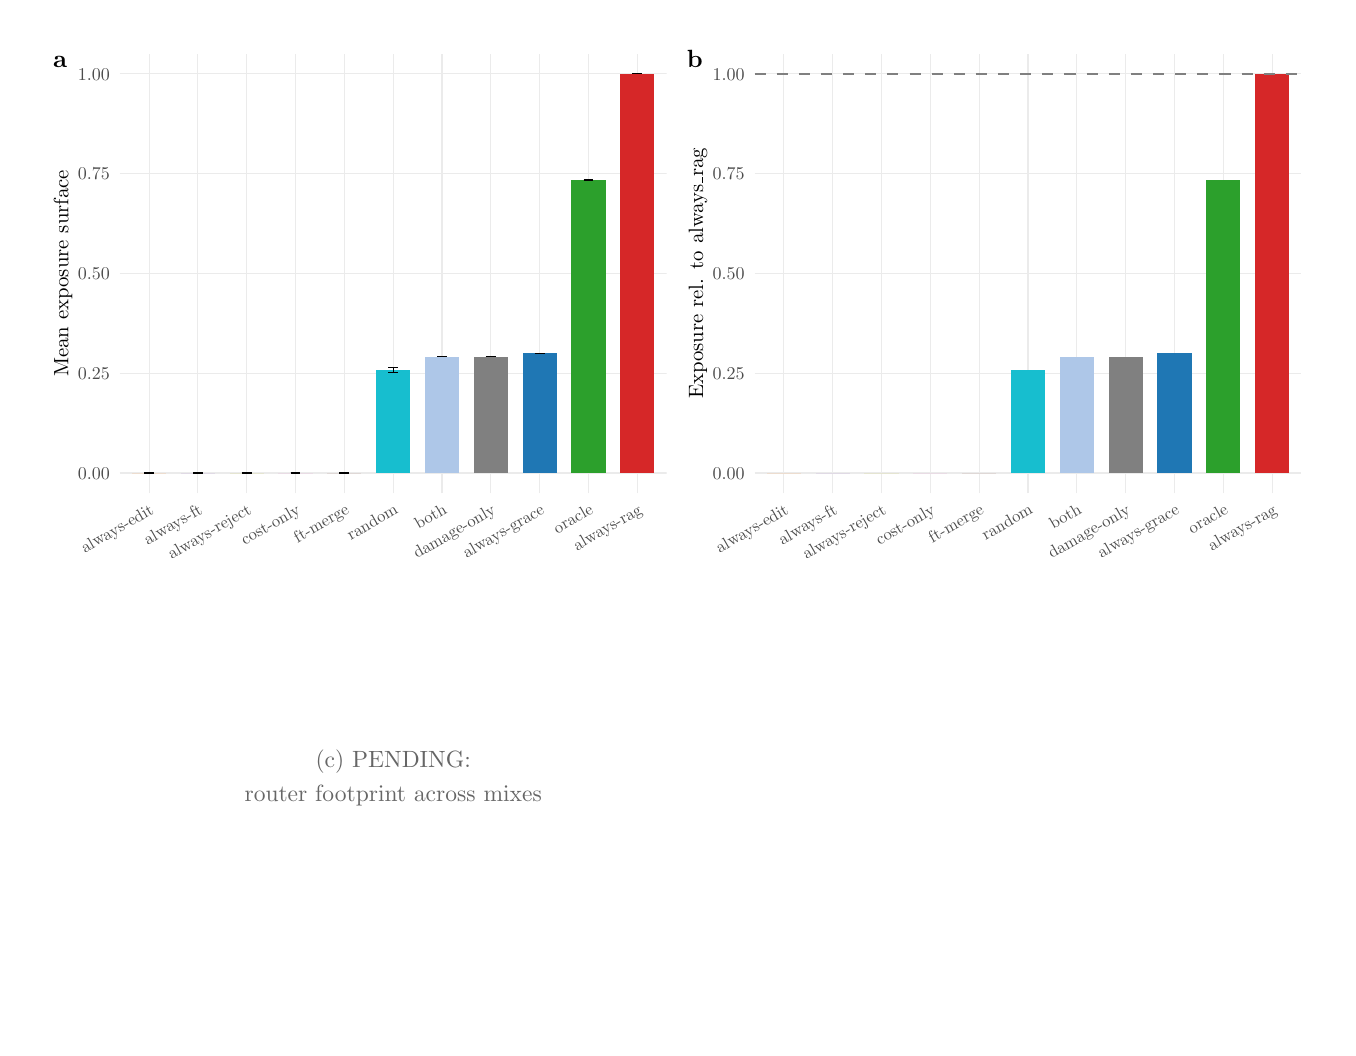
\begin{tikzpicture}[x=1pt,y=1pt]
\definecolor{fillColor}{RGB}{255,255,255}
\path[use as bounding box,fill=fillColor,fill opacity=0.00] (0,0) rectangle (469.75,361.35);
\begin{scope}
\path[clip] (  0.00,  0.00) rectangle (469.75,361.35);
\definecolor{drawColor}{RGB}{255,255,255}
\definecolor{fillColor}{RGB}{255,255,255}

\path[draw=drawColor,line width= 0.6pt,line join=round,line cap=round,fill=fillColor] (  0.00,  0.00) rectangle (469.75,361.35);
\end{scope}
\begin{scope}
\path[clip] (  5.50,164.15) rectangle (234.88,355.85);
\definecolor{fillColor}{RGB}{255,255,255}

\path[fill=fillColor] (  5.50,164.15) rectangle (234.88,355.85);
\end{scope}
\begin{scope}
\path[clip] (234.88,164.15) rectangle (464.25,355.85);
\definecolor{fillColor}{RGB}{255,255,255}

\path[fill=fillColor] (234.88,164.15) rectangle (464.25,355.85);
\end{scope}
\begin{scope}
\path[clip] (  5.50,  5.50) rectangle (234.88,164.15);

\path[] (  5.50,  5.50) rectangle (234.88,164.15);
\end{scope}
\begin{scope}
\path[clip] (234.88,  5.50) rectangle (464.25,164.15);

\path[] (234.88,  5.50) rectangle (464.25,164.15);
\end{scope}
\begin{scope}
\path[clip] ( 33.28,193.20) rectangle (230.88,351.85);
\definecolor{drawColor}{gray}{0.92}

\path[draw=drawColor,line width= 0.4pt,line join=round] ( 33.28,200.41) --
	(230.88,200.41);

\path[draw=drawColor,line width= 0.4pt,line join=round] ( 33.28,236.47) --
	(230.88,236.47);

\path[draw=drawColor,line width= 0.4pt,line join=round] ( 33.28,272.52) --
	(230.88,272.52);

\path[draw=drawColor,line width= 0.4pt,line join=round] ( 33.28,308.58) --
	(230.88,308.58);

\path[draw=drawColor,line width= 0.4pt,line join=round] ( 33.28,344.64) --
	(230.88,344.64);

\path[draw=drawColor,line width= 0.4pt,line join=round] ( 43.86,193.20) --
	( 43.86,351.85);

\path[draw=drawColor,line width= 0.4pt,line join=round] ( 61.50,193.20) --
	( 61.50,351.85);

\path[draw=drawColor,line width= 0.4pt,line join=round] ( 79.15,193.20) --
	( 79.15,351.85);

\path[draw=drawColor,line width= 0.4pt,line join=round] ( 96.79,193.20) --
	( 96.79,351.85);

\path[draw=drawColor,line width= 0.4pt,line join=round] (114.43,193.20) --
	(114.43,351.85);

\path[draw=drawColor,line width= 0.4pt,line join=round] (132.08,193.20) --
	(132.08,351.85);

\path[draw=drawColor,line width= 0.4pt,line join=round] (149.72,193.20) --
	(149.72,351.85);

\path[draw=drawColor,line width= 0.4pt,line join=round] (167.36,193.20) --
	(167.36,351.85);

\path[draw=drawColor,line width= 0.4pt,line join=round] (185.01,193.20) --
	(185.01,351.85);

\path[draw=drawColor,line width= 0.4pt,line join=round] (202.65,193.20) --
	(202.65,351.85);

\path[draw=drawColor,line width= 0.4pt,line join=round] (220.29,193.20) --
	(220.29,351.85);
\definecolor{fillColor}{RGB}{255,127,14}

\path[fill=fillColor] ( 37.69,200.41) rectangle ( 50.04,200.41);
\definecolor{fillColor}{RGB}{148,103,189}

\path[fill=fillColor] ( 55.33,200.41) rectangle ( 67.68,200.41);
\definecolor{fillColor}{RGB}{31,119,180}

\path[fill=fillColor] (178.83,200.41) rectangle (191.18,243.68);
\definecolor{fillColor}{RGB}{214,39,40}

\path[fill=fillColor] (214.12,200.41) rectangle (226.47,344.64);
\definecolor{fillColor}{RGB}{188,189,34}

\path[fill=fillColor] ( 72.97,200.41) rectangle ( 85.32,200.41);
\definecolor{fillColor}{RGB}{174,199,232}

\path[fill=fillColor] (143.54,200.41) rectangle (155.89,242.47);
\definecolor{fillColor}{RGB}{227,119,194}

\path[fill=fillColor] ( 90.62,200.41) rectangle (102.97,200.41);
\definecolor{fillColor}{gray}{0.50}

\path[fill=fillColor] (161.19,200.41) rectangle (173.54,242.47);
\definecolor{fillColor}{RGB}{140,86,75}

\path[fill=fillColor] (108.26,200.41) rectangle (120.61,200.41);
\definecolor{fillColor}{RGB}{44,160,44}

\path[fill=fillColor] (196.47,200.41) rectangle (208.82,306.21);
\definecolor{fillColor}{RGB}{23,190,207}

\path[fill=fillColor] (125.90,200.41) rectangle (138.25,237.57);
\definecolor{drawColor}{RGB}{0,0,0}

\path[draw=drawColor,line width= 0.4pt,line join=round] ( 42.10,200.41) --
	( 45.63,200.41);

\path[draw=drawColor,line width= 0.4pt,line join=round] ( 43.86,200.41) --
	( 43.86,200.41);

\path[draw=drawColor,line width= 0.4pt,line join=round] ( 42.10,200.41) --
	( 45.63,200.41);

\path[draw=drawColor,line width= 0.4pt,line join=round] ( 59.74,200.41) --
	( 63.27,200.41);

\path[draw=drawColor,line width= 0.4pt,line join=round] ( 61.50,200.41) --
	( 61.50,200.41);

\path[draw=drawColor,line width= 0.4pt,line join=round] ( 59.74,200.41) --
	( 63.27,200.41);

\path[draw=drawColor,line width= 0.4pt,line join=round] (183.24,243.68) --
	(186.77,243.68);

\path[draw=drawColor,line width= 0.4pt,line join=round] (185.01,243.68) --
	(185.01,243.68);

\path[draw=drawColor,line width= 0.4pt,line join=round] (183.24,243.68) --
	(186.77,243.68);

\path[draw=drawColor,line width= 0.4pt,line join=round] (218.53,344.64) --
	(222.06,344.64);

\path[draw=drawColor,line width= 0.4pt,line join=round] (220.29,344.64) --
	(220.29,344.64);

\path[draw=drawColor,line width= 0.4pt,line join=round] (218.53,344.64) --
	(222.06,344.64);

\path[draw=drawColor,line width= 0.4pt,line join=round] ( 77.38,200.41) --
	( 80.91,200.41);

\path[draw=drawColor,line width= 0.4pt,line join=round] ( 79.15,200.41) --
	( 79.15,200.41);

\path[draw=drawColor,line width= 0.4pt,line join=round] ( 77.38,200.41) --
	( 80.91,200.41);

\path[draw=drawColor,line width= 0.4pt,line join=round] (147.96,242.47) --
	(151.48,242.47);

\path[draw=drawColor,line width= 0.4pt,line join=round] (149.72,242.47) --
	(149.72,242.47);

\path[draw=drawColor,line width= 0.4pt,line join=round] (147.96,242.47) --
	(151.48,242.47);

\path[draw=drawColor,line width= 0.4pt,line join=round] ( 95.03,200.41) --
	( 98.56,200.41);

\path[draw=drawColor,line width= 0.4pt,line join=round] ( 96.79,200.41) --
	( 96.79,200.41);

\path[draw=drawColor,line width= 0.4pt,line join=round] ( 95.03,200.41) --
	( 98.56,200.41);

\path[draw=drawColor,line width= 0.4pt,line join=round] (165.60,242.47) --
	(169.13,242.47);

\path[draw=drawColor,line width= 0.4pt,line join=round] (167.36,242.47) --
	(167.36,242.47);

\path[draw=drawColor,line width= 0.4pt,line join=round] (165.60,242.47) --
	(169.13,242.47);

\path[draw=drawColor,line width= 0.4pt,line join=round] (112.67,200.41) --
	(116.20,200.41);

\path[draw=drawColor,line width= 0.4pt,line join=round] (114.43,200.41) --
	(114.43,200.41);

\path[draw=drawColor,line width= 0.4pt,line join=round] (112.67,200.41) --
	(116.20,200.41);

\path[draw=drawColor,line width= 0.4pt,line join=round] (200.88,306.32) --
	(204.41,306.32);

\path[draw=drawColor,line width= 0.4pt,line join=round] (202.65,306.32) --
	(202.65,306.09);

\path[draw=drawColor,line width= 0.4pt,line join=round] (200.88,306.09) --
	(204.41,306.09);

\path[draw=drawColor,line width= 0.4pt,line join=round] (130.31,238.53) --
	(133.84,238.53);

\path[draw=drawColor,line width= 0.4pt,line join=round] (132.08,238.53) --
	(132.08,236.61);

\path[draw=drawColor,line width= 0.4pt,line join=round] (130.31,236.61) --
	(133.84,236.61);
\end{scope}
\begin{scope}
\path[clip] (  0.00,  0.00) rectangle (469.75,361.35);
\definecolor{drawColor}{gray}{0.30}

\node[text=drawColor,anchor=base east,inner sep=0pt, outer sep=0pt, scale=  0.65] at ( 29.68,198.17) {0.00};

\node[text=drawColor,anchor=base east,inner sep=0pt, outer sep=0pt, scale=  0.65] at ( 29.68,234.23) {0.25};

\node[text=drawColor,anchor=base east,inner sep=0pt, outer sep=0pt, scale=  0.65] at ( 29.68,270.28) {0.50};

\node[text=drawColor,anchor=base east,inner sep=0pt, outer sep=0pt, scale=  0.65] at ( 29.68,306.34) {0.75};

\node[text=drawColor,anchor=base east,inner sep=0pt, outer sep=0pt, scale=  0.65] at ( 29.68,342.40) {1.00};
\end{scope}
\begin{scope}
\path[clip] (  0.00,  0.00) rectangle (469.75,361.35);
\definecolor{drawColor}{gray}{0.30}

\node[text=drawColor,rotate= 30.00,anchor=base east,inner sep=0pt, outer sep=0pt, scale=  0.60] at ( 45.93,186.02) {always-edit};

\node[text=drawColor,rotate= 30.00,anchor=base east,inner sep=0pt, outer sep=0pt, scale=  0.60] at ( 63.57,186.02) {always-ft};

\node[text=drawColor,rotate= 30.00,anchor=base east,inner sep=0pt, outer sep=0pt, scale=  0.60] at ( 81.21,186.02) {always-reject};

\node[text=drawColor,rotate= 30.00,anchor=base east,inner sep=0pt, outer sep=0pt, scale=  0.60] at ( 98.86,186.02) {cost-only};

\node[text=drawColor,rotate= 30.00,anchor=base east,inner sep=0pt, outer sep=0pt, scale=  0.60] at (116.50,186.02) {ft-merge};

\node[text=drawColor,rotate= 30.00,anchor=base east,inner sep=0pt, outer sep=0pt, scale=  0.60] at (134.14,186.02) {random};

\node[text=drawColor,rotate= 30.00,anchor=base east,inner sep=0pt, outer sep=0pt, scale=  0.60] at (151.79,186.02) {both};

\node[text=drawColor,rotate= 30.00,anchor=base east,inner sep=0pt, outer sep=0pt, scale=  0.60] at (169.43,186.02) {damage-only};

\node[text=drawColor,rotate= 30.00,anchor=base east,inner sep=0pt, outer sep=0pt, scale=  0.60] at (187.07,186.02) {always-grace};

\node[text=drawColor,rotate= 30.00,anchor=base east,inner sep=0pt, outer sep=0pt, scale=  0.60] at (204.71,186.02) {oracle};

\node[text=drawColor,rotate= 30.00,anchor=base east,inner sep=0pt, outer sep=0pt, scale=  0.60] at (222.36,186.02) {always-rag};
\end{scope}
\begin{scope}
\path[clip] (  0.00,  0.00) rectangle (469.75,361.35);
\definecolor{drawColor}{RGB}{0,0,0}

\node[text=drawColor,rotate= 90.00,anchor=base,inner sep=0pt, outer sep=0pt, scale=  0.75] at ( 14.67,272.52) {Mean exposure surface};
\end{scope}
\begin{scope}
\path[clip] (  0.00,  0.00) rectangle (469.75,361.35);
\definecolor{drawColor}{RGB}{0,0,0}

\node[text=drawColor,anchor=base,inner sep=0pt, outer sep=0pt, scale=  0.90] at ( 11.71,346.91) {\bfseries a};
\end{scope}
\begin{scope}
\path[clip] (262.65,193.20) rectangle (460.25,351.85);
\definecolor{drawColor}{gray}{0.92}

\path[draw=drawColor,line width= 0.4pt,line join=round] (262.65,200.41) --
	(460.25,200.41);

\path[draw=drawColor,line width= 0.4pt,line join=round] (262.65,236.47) --
	(460.25,236.47);

\path[draw=drawColor,line width= 0.4pt,line join=round] (262.65,272.52) --
	(460.25,272.52);

\path[draw=drawColor,line width= 0.4pt,line join=round] (262.65,308.58) --
	(460.25,308.58);

\path[draw=drawColor,line width= 0.4pt,line join=round] (262.65,344.64) --
	(460.25,344.64);

\path[draw=drawColor,line width= 0.4pt,line join=round] (273.24,193.20) --
	(273.24,351.85);

\path[draw=drawColor,line width= 0.4pt,line join=round] (290.88,193.20) --
	(290.88,351.85);

\path[draw=drawColor,line width= 0.4pt,line join=round] (308.53,193.20) --
	(308.53,351.85);

\path[draw=drawColor,line width= 0.4pt,line join=round] (326.17,193.20) --
	(326.17,351.85);

\path[draw=drawColor,line width= 0.4pt,line join=round] (343.81,193.20) --
	(343.81,351.85);

\path[draw=drawColor,line width= 0.4pt,line join=round] (361.45,193.20) --
	(361.45,351.85);

\path[draw=drawColor,line width= 0.4pt,line join=round] (379.10,193.20) --
	(379.10,351.85);

\path[draw=drawColor,line width= 0.4pt,line join=round] (396.74,193.20) --
	(396.74,351.85);

\path[draw=drawColor,line width= 0.4pt,line join=round] (414.38,193.20) --
	(414.38,351.85);

\path[draw=drawColor,line width= 0.4pt,line join=round] (432.03,193.20) --
	(432.03,351.85);

\path[draw=drawColor,line width= 0.4pt,line join=round] (449.67,193.20) --
	(449.67,351.85);
\definecolor{fillColor}{RGB}{255,127,14}

\path[fill=fillColor] (267.06,200.41) rectangle (279.41,200.41);
\definecolor{fillColor}{RGB}{148,103,189}

\path[fill=fillColor] (284.71,200.41) rectangle (297.06,200.41);
\definecolor{fillColor}{RGB}{31,119,180}

\path[fill=fillColor] (408.21,200.41) rectangle (420.56,243.68);
\definecolor{fillColor}{RGB}{214,39,40}

\path[fill=fillColor] (443.49,200.41) rectangle (455.84,344.64);
\definecolor{fillColor}{RGB}{188,189,34}

\path[fill=fillColor] (302.35,200.41) rectangle (314.70,200.41);
\definecolor{fillColor}{RGB}{174,199,232}

\path[fill=fillColor] (372.92,200.41) rectangle (385.27,242.47);
\definecolor{fillColor}{RGB}{227,119,194}

\path[fill=fillColor] (319.99,200.41) rectangle (332.34,200.41);
\definecolor{fillColor}{gray}{0.50}

\path[fill=fillColor] (390.57,200.41) rectangle (402.92,242.47);
\definecolor{fillColor}{RGB}{140,86,75}

\path[fill=fillColor] (337.64,200.41) rectangle (349.99,200.41);
\definecolor{fillColor}{RGB}{44,160,44}

\path[fill=fillColor] (425.85,200.41) rectangle (438.20,306.21);
\definecolor{fillColor}{RGB}{23,190,207}

\path[fill=fillColor] (355.28,200.41) rectangle (367.63,237.57);
\definecolor{drawColor}{gray}{0.50}

\path[draw=drawColor,line width= 0.5pt,dash pattern=on 4pt off 4pt ,line join=round] (262.65,344.64) -- (460.25,344.64);
\end{scope}
\begin{scope}
\path[clip] (  0.00,  0.00) rectangle (469.75,361.35);
\definecolor{drawColor}{gray}{0.30}

\node[text=drawColor,anchor=base east,inner sep=0pt, outer sep=0pt, scale=  0.65] at (259.05,198.17) {0.00};

\node[text=drawColor,anchor=base east,inner sep=0pt, outer sep=0pt, scale=  0.65] at (259.05,234.23) {0.25};

\node[text=drawColor,anchor=base east,inner sep=0pt, outer sep=0pt, scale=  0.65] at (259.05,270.28) {0.50};

\node[text=drawColor,anchor=base east,inner sep=0pt, outer sep=0pt, scale=  0.65] at (259.05,306.34) {0.75};

\node[text=drawColor,anchor=base east,inner sep=0pt, outer sep=0pt, scale=  0.65] at (259.05,342.40) {1.00};
\end{scope}
\begin{scope}
\path[clip] (  0.00,  0.00) rectangle (469.75,361.35);
\definecolor{drawColor}{gray}{0.30}

\node[text=drawColor,rotate= 30.00,anchor=base east,inner sep=0pt, outer sep=0pt, scale=  0.60] at (275.31,186.02) {always-edit};

\node[text=drawColor,rotate= 30.00,anchor=base east,inner sep=0pt, outer sep=0pt, scale=  0.60] at (292.95,186.02) {always-ft};

\node[text=drawColor,rotate= 30.00,anchor=base east,inner sep=0pt, outer sep=0pt, scale=  0.60] at (310.59,186.02) {always-reject};

\node[text=drawColor,rotate= 30.00,anchor=base east,inner sep=0pt, outer sep=0pt, scale=  0.60] at (328.23,186.02) {cost-only};

\node[text=drawColor,rotate= 30.00,anchor=base east,inner sep=0pt, outer sep=0pt, scale=  0.60] at (345.88,186.02) {ft-merge};

\node[text=drawColor,rotate= 30.00,anchor=base east,inner sep=0pt, outer sep=0pt, scale=  0.60] at (363.52,186.02) {random};

\node[text=drawColor,rotate= 30.00,anchor=base east,inner sep=0pt, outer sep=0pt, scale=  0.60] at (381.16,186.02) {both};

\node[text=drawColor,rotate= 30.00,anchor=base east,inner sep=0pt, outer sep=0pt, scale=  0.60] at (398.81,186.02) {damage-only};

\node[text=drawColor,rotate= 30.00,anchor=base east,inner sep=0pt, outer sep=0pt, scale=  0.60] at (416.45,186.02) {always-grace};

\node[text=drawColor,rotate= 30.00,anchor=base east,inner sep=0pt, outer sep=0pt, scale=  0.60] at (434.09,186.02) {oracle};

\node[text=drawColor,rotate= 30.00,anchor=base east,inner sep=0pt, outer sep=0pt, scale=  0.60] at (451.74,186.02) {always-rag};
\end{scope}
\begin{scope}
\path[clip] (  0.00,  0.00) rectangle (469.75,361.35);
\definecolor{drawColor}{RGB}{0,0,0}

\node[text=drawColor,rotate= 90.00,anchor=base,inner sep=0pt, outer sep=0pt, scale=  0.75] at (244.04,272.52) {Exposure rel. to always\_rag};
\end{scope}
\begin{scope}
\path[clip] (  0.00,  0.00) rectangle (469.75,361.35);
\definecolor{drawColor}{RGB}{0,0,0}

\node[text=drawColor,anchor=base,inner sep=0pt, outer sep=0pt, scale=  0.90] at (241.09,346.91) {\bfseries b};
\end{scope}
\begin{scope}
\path[clip] ( 33.28,  5.50) rectangle (230.88,164.15);
\definecolor{drawColor}{gray}{0.40}

\node[text=drawColor,anchor=base,inner sep=0pt, outer sep=0pt, scale=  0.85] at (132.08, 94.18) {(c) PENDING:};

\node[text=drawColor,anchor=base,inner sep=0pt, outer sep=0pt, scale=  0.85] at (132.08, 81.89) {router footprint across mixes};
\end{scope}
\end{tikzpicture}
